% !TEX encoding = UTF-8 Unicode
\documentclass[11pt, a4paper, oneside]{article}
\usepackage[onehalfspacing]{setspace}		% One half spacing
\usepackage{hyperref}					% Hyperlinks on pdf (Should be called before Geometry)
\usepackage[a4paper, 					% Page Layout
                     %showframe,				% This shows the frame
                     twoside, includehead,
                     footskip=7mm, headsep=6mm, headheight=4.8mm,
                     marginparsep=2mm, marginparwidth=22mm,
                     top=25mm, bottom=25mm, inner=30mm, outer=25mm]{geometry}
\usepackage{sansmathfonts}				% Sans Serif equations
\usepackage[T1]{fontenc}					% Output font encoding for international characters
\usepackage[utf8]{inputenc}				% Encoding of files: utf8
\renewcommand*\familydefault{\sfdefault} 		% Sans Serif as default font
\usepackage[table]{xcolor}
\usepackage{graphicx}
\usepackage{pdfpages}
\usepackage{array}
\hypersetup{
    colorlinks=true,
    linkcolor=blue,
    filecolor=magenta,      
    urlcolor=blue,
}
\urlstyle{same}
\usepackage{tikz}
\RequirePackage{caption} 				% Caption customization
\captionsetup{justification=centerlast,font=small,labelfont=sc,margin=1cm}

\usepackage{array}
\newcommand{\PreserveBackslash}[1]{\let\temp=\\#1\let\\=\temp}
\newcolumntype{C}[1]{>{\PreserveBackslash\centering}p{#1}}
\newcolumntype{R}[1]{>{\PreserveBackslash\raggedleft}p{#1}}
\newcolumntype{L}[1]{>{\PreserveBackslash\raggedright}p{#1}}

\begin{document}
\begin{titlepage}
	\onehalfspacing
	\enlargethispage{0.65\baselineskip}
	\begin{tikzpicture}[remember picture, overlay]
		\coordinate (top_right) at 
		    ([xshift=-2.5cm, yshift=-2.5cm]current page.north east);
		\coordinate (top_left) at 
		    ([xshift=2.3cm, yshift=-1.8cm]current page.north west);
		\coordinate (bottom_right) at 
		    ([xshift=-1.8cm, yshift=1.8cm]current page.south east);
		\node[inner sep=0, anchor=north east] at (top_right) {\href{http://www.itba.edu.ar}{
\includegraphics[height=19mm, trim={180 200 200 200}, clip]{figs/logo_itba.png}}};
		\draw[double, line width = 0.5pt] (top_left) rectangle (bottom_right);
	\end{tikzpicture}
	\par
	\vspace{-0.8cm}
	\noindent \textbf{CENTRO DE INVESTIGACIÓN Y DESARROLLO EN}\par
	\noindent \textbf{ELECTRONICA INDUSTRIAL (CIDEI)}\par
	\vspace{3cm}
	\begin{center}
		{\Huge \textbf{ARiCE Plattform}\par}
		{\huge \textbf{Getting Started Radiant}\par}
	\end{center}
	\vspace{1cm}
	\begin{center}
		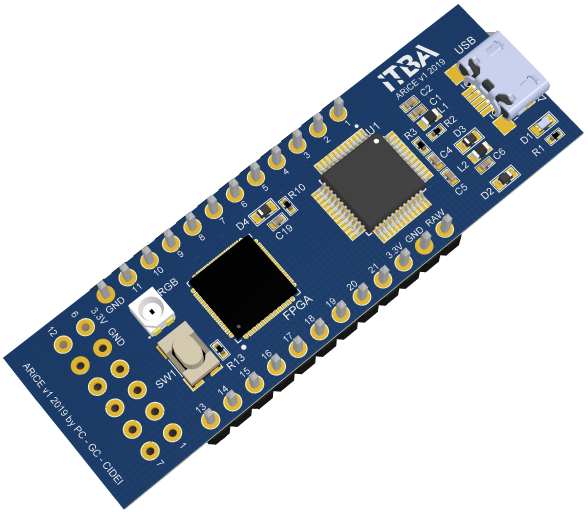
\includegraphics[width=8cm]{figs/fig1a.png}
	\end{center}
	\vfill
	\noindent \textbf{AUTHORS:} Dr. Ing. Pablo \textsc{Cossutta} - Ing. Gonzalo \textsc{Castelli} \par
	\vfill
	\begin{center}
		\textbf{CIUDAD AUTÓNOMA DE BUENOS AIRES}\\
		\textbf{2018-2019}\par
	\end{center}
\end{titlepage}

\tableofcontents
\newpage

\section{Introduction}
This project is an open-source platform,shown on Fig. \ref{fig1},  based on a low cost and low consumption FPGA chip from \href{http://www.latticesemi.com}{Lattice Semiconductor}, aiming to be used in a wide range of signal processing and control applications, both for education and the industry.
%
\begin{figure}[h!]
	\centering
	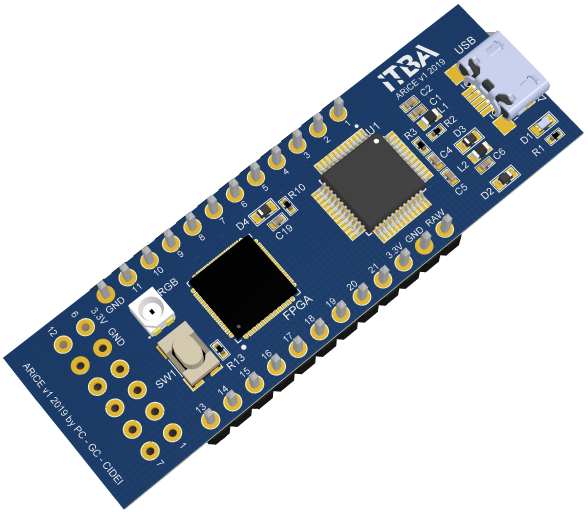
\includegraphics[width=8cm]{figs/fig1a.png}\\
	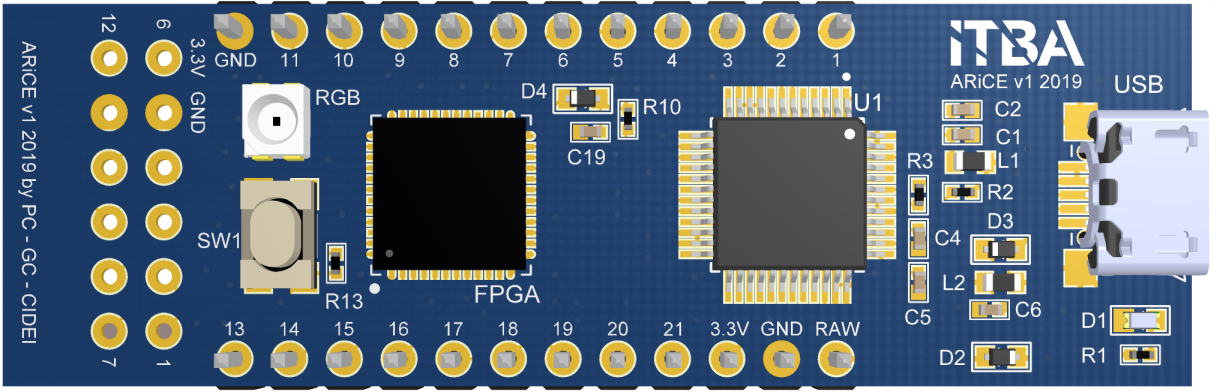
\includegraphics[width=6cm]{figs/fig1b.png}%
	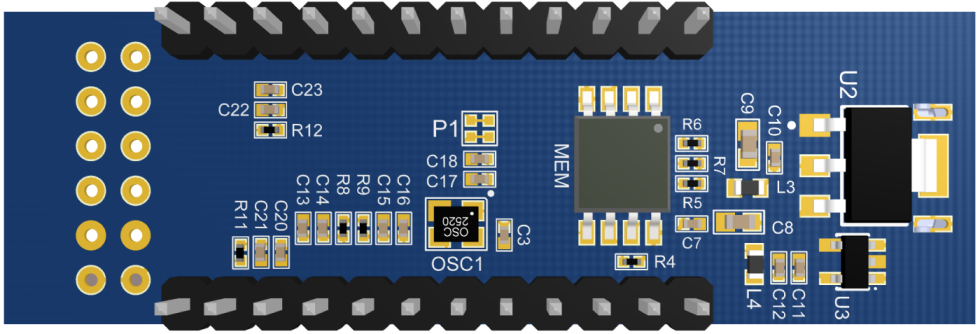
\includegraphics[width=6cm]{figs/fig1c.png}
	\caption{Board's view}
	\label{fig1}
\end{figure}

%\subsection{Project file sources}
%The following list shows the different file sources for this project:
%\begin{itemize}
%	\item Getting Started Guide and Documentation: \href{https://github.com/pcossutta/Lattice-FPGA/tree/master/Documents/Manuals}{GitHub manuals}
%	\item PCB and Schematics: \href{https://workspace.circuitmaker.com/Projects/Details/Gonzalo-Castelli/FPGA-ITBA}{Circuit Maker} and \href{https://github.com/pcossutta/Lattice-FPGA/tree/master/Altium}{GitHub Altium Project Files}
%	\item \href{https://github.com/pcossutta/Lattice-FPGA/tree/master/Examples/LedExample}{Example code} for the Lattice Radiant software.
%\end{itemize}

\section{Getting started}
Three main steps are necessary to use the board if you are starting from scratch. The first is to download the software and get a license, the second is to create a new project and include the code files needed and finally load the program to the onboard memory using a USB cable.

\subsection{Download the software}
Before using the board, it is necessary to set up the software to program the Lattice iCE40-UP5K FPGA chip. It is recommended to use \href{http://www.latticesemi.com/Products/DesignSoftwareAndIP/FPGAandLDS/Radiant}{Lattice Radiant software}, which supports iCE40 UltraPlus and offers all the best in class tools and features to develop edge applications effectively and efficiently. Free registration is required to download the software, and a license can be requested with no charge after providing the MAC address of the computer it will run on. 
This development also supports the \href{http://www.clifford.at/icestorm/}{iceStorm project}, Open Source toolchain by Clifford Wolf although its usage is not covered in this document.

\subsection{Create a new project}
After having installed and licensed the software, the next step is to create a new project in the Lattice Radiant Software and start writing HDL code. An example code that uses the onboard RGB LED is available for download at the GitHub repository of this project. After downloading the files, open the Lattice Radiant application and go to:
\begin{center}
	File $\rightarrow$ Open $\rightarrow$ Project...
\end{center}
Browse the folder you downloaded from GitHub and select the \texttt{getting\_started.rdf} file. You can now jump to the next section. To learn how to manually create a new project, click on the "New Project" icon in the start page, or by going to:
\begin{center}
	File $\rightarrow$ New $\rightarrow$ Project...
\end{center}
Follow the instructions of the wizard, and name the project "getting\_started". After clicking "Next", a new window will ask for source files. Click the "Add Source..." button and load the Verilog File you downloaded from the GitHub repository called "top.v". Check both boxes at the bottom of the window to generate all the necessary files in the project folder. The window should look like Fig. \ref{fig2}.
%
\begin{figure}[h!]
	\centering
	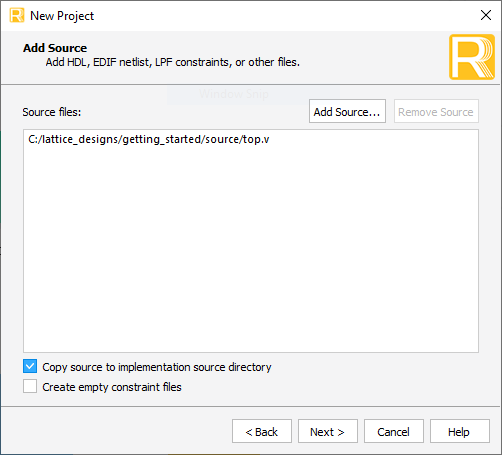
\includegraphics[scale=0.8]{figs/fig2.png}
	\caption{Adding source files to the new project}
	\label{fig2}
\end{figure}

Click "Next", and select the "iCE40UP5K" device. In the package pull-down menu, choose "SG48" and in the Part Number menu, pick "iCE40UP5K-SG48I". The window should look like Fig. \ref{fig3}.

\begin{figure}[h!]
	\centering
	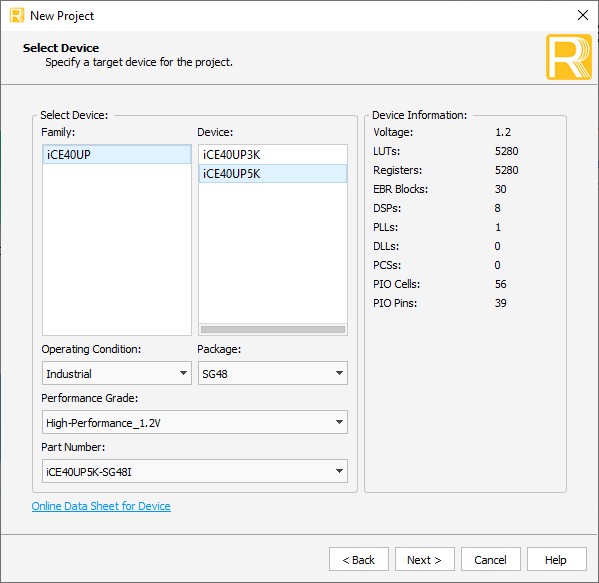
\includegraphics[scale=0.71]{figs/fig3.png}
	\caption{Selecting the device}
	\label{fig3}
\end{figure}

Then, click "Next" and "Finish" to conclude with the wizard. Now, replace the content of the \texttt{impl\_1.ldc}  and \texttt{impl\_1.pdc} files with the ones from our example in the GitHub repository. The project has now been set up, and the last step remaining is to load the code to the memory of the board.

\subsection{Board Programming}
Now that the project is fully set up, it is necessary to synthesize the design to create the export files. Click on the green play button on the upper-left corner to do so. The process should succeed, even though warnings will appear. Connect the FPGA board to the PC using the USB cable. To set up the device for programming, go to:
\begin{center}
	Tools $\rightarrow$ Programmer
\end{center}
In the Radiant Programmer window, the iCE40UP5K device should be displayed in the list. Select it by clicking on it, and go to:
\begin{center}
	Edit $\rightarrow$ Device Properties...
\end{center}
Configure the window so it looks like Fig. \ref{fig4}. Do not forget to include the programming file path, which was generated when doing the synthesis and which has a ".bin" extension. In our case, the file is \texttt{getting\_started\_impl1.bin}.

\begin{figure}[h!]
    \centering
    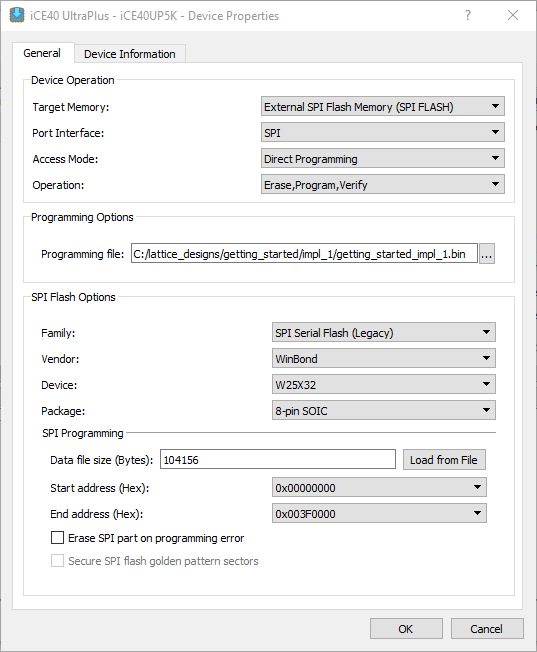
\includegraphics[scale=0.8]{figs/fig4.png}
    \caption{Programming properties}
    \label{fig4}
\end{figure}

Click "OK" to exit the window and to finally load the program to the board's memory go to:
\begin{center}
 Run $\rightarrow$ Program Device
\end{center}
If done successfully, the RGB LED of the FPGA board should be flashing in colors. 

% !TEX encoding = UTF-8 Unicode
\newpage
\section{Pinout information}
The board has multiple I/O pins, as well as power supply pins, distributed along the side and the front of the PCB. The next list gives a short description of the signals:
\begin{itemize}
	\item IOT\_XX are general I/O pins. In user mode, after configuration, these pins can be programmed as I/O in user function in the top (xx = I/O location)
	\item IOB\_XX are general I/O pins. In user mode, after configuration, these pins can be programmed as I/O in user function in the bottom (xx = I/O location)
	\item RAW VCC. The input voltage to the FPGA board when it's using an external power source. The board can be supplied with power either from the USB connector or the RAW VCC pin. The nominal supply voltage is 5V. (Minimum is 4.5V and maximum is 6V)
	\item 3.3V. A 3.3 volt supply generated by the on-board regulator. Maximum recommended current draw from this pin is 500 mA
	\item GND. Ground pins
	\item Signal names with G1, G3 and G6 suffixes may be used as a General I/O or as a Global input used for high fanout, or clock/reset net. These pins drive the GBUF1, GBUF3 and GBUF6 global buffers respectively
\end{itemize}

\newpage
Table \ref{table1} shows the mapping between the signals and the board pin numbers.
\definecolor{myHdr}{rgb}{0.81000,0.8800,0.9400}%
\begin{table}[h!]
	\renewcommand{\arraystretch}{1.3}
	\caption{Connections}
	\label{table1}
	\begin{tabular}[t]{C{0.12\textwidth} C{0.12\textwidth} C{0.15\textwidth}}
		\bfseries Board Pin & \bfseries FPGA Pin & \bfseries Signal Name \\ \hline
		\rowcolor{myHdr} \multicolumn{3}{c}{\bfseries Side Pins} \\ \hline
		1 & 20 & IOB 25B G3 \\
		2 & 21 & IOB 23B \\
		3 & 23 & IOT 37A \\
		4 & 25 & IOT 36B \\
		5 & 26 & IOT 39A \\
		6 & 27 & IOT 38B \\
		7 & 31 & IOT 42B \\
		8 & 32 & IOT 43A \\
		9 & 34 & IOT 44B \\
		10 & 36 & IOT 48B \\
		11 & 37 & IOT 45A G1 \\
		12 & - & GND \\
		& & \\
		13 & 2 & IOB 6A \\
		14 & 6 & IOB 13B \\
		15 & 9 & IOB 16A \\
		16 & 10 & IOB 18A \\
		17 & 11 & IOB 20A \\
		18 & 12 & IOB 22A \\
		19 & 13 & IOB 24A \\
		20 & 18 & IOB 31B \\
		21 & 19 & IOB 29B \\
		22 & - & 3.3V \\
		23 & - & GND \\
		24 & - & RAW VCC \\
	\end{tabular}
	\quad
	\begin{tabular}[t]{C{0.12\textwidth} C{0.12\textwidth} C{0.15\textwidth}}
		\bfseries Board Pin & \bfseries FPGA Pin & \bfseries Signal Name \\ \hline
		\rowcolor{myHdr} \multicolumn{3}{c}{\bfseries Front Pins} \\ \hline
		1 & 4 & IOB 8A \\
		2 & 3 & IOB 9B \\
		3 & 47 & IOB 2A \\
		4 & 44 & IOB 3B G6 \\
		5 & - & GND \\
		6 & - & 3.3V \\
		7 & 48 & IOB 4A \\
		8 & 45 & IOB 5B \\
		9 & 38 & IOT 50B \\
		10 & 42 & IOT 51A \\
		11 & - & GND \\
		12 & - & 3.3V \\
		& & \\
		\bfseries Board Pin & \bfseries FPGA Pin & \bfseries Signal Name \\ \hline
		\rowcolor{myHdr} \multicolumn{3}{c}{\bfseries Not Connected} \\ \hline
		 - & 43 & IOT 49A \\
		- & 46 & IOB 0A \\
		- & 28 & IOT 41A \\	
		& & \\
		& & \\
		\bfseries LED Color & \bfseries FPGA Pin & \bfseries Signal Name \\ \hline
		\rowcolor{myHdr} \multicolumn{3}{c}{\bfseries Onboard RGB LED} \\   \hline
		Blue & 39 & RGB0 \\
		Green & 40 & RGB1 \\
		Red & 41 & RGB2 \\
	\end{tabular}
\end{table}

\newpage
The differential pairs are shown in Table \ref{table2}. They are grouped together and labeled in colors, white is positive and light blue is negative.
%
\begin{table}[h!]
	\renewcommand{\arraystretch}{1.3}
	\caption{Differential Pairs}
	\vspace{0.5em}
	\label{table2}
	\centering
	\begin{tabular}{C{0.12\textwidth} C{0.12\textwidth} C{0.15\textwidth}}
		\bfseries Board Pin & \bfseries FPGA Pin & \bfseries Signal Name \\ \hline
		\rowcolor{myHdr}  3 & 23 & IOT 37A \\
		4 & 25 & IOT 36B \\ \hline
		\rowcolor{myHdr}  5 & 26 & IOT 39A \\
		6 & 27 & IOT 38B \\ \hline
		\rowcolor{myHdr}  8 & 32 & IOT 43A \\
		7 & 31 & IOT 42B \\ \hline
		\rowcolor{myHdr}  11 & 37 & IOT 45A G1 \\
		9 & 34 & IOT 44B \\ \hline
		\rowcolor{myHdr}  2 & 21 & IOB 23B \\
		18 & 12 & IOB 22A \\ \hline
		\rowcolor{myHdr}  2 & 3 & IOB 9B \\
		1 & 4 & IOB 8A \\ \hline
		\rowcolor{myHdr}  4 & 44 & IOB 3B G6 \\
		3 & 47 & IOB 2A \\ \hline
		\rowcolor{myHdr}  8 & 45 & IOB 5B \\ 
		7 & 48 & IOB 4A \\ \hline
		\rowcolor{myHdr}  10 & 42 & IOT 51A \\ 
		9 & 38 & IOT 50B \\
	\end{tabular}
\end{table}

\section{Open Source PCB}
The board files, circuit schematics and list of components are available in the GitHub repository. Altium project and Gerber files are available. The board is also published in open source EDAs just as \href{https://workspace.circuitmaker.com/}{Circuit Maker} and \href{http://www.kicad-pcb.org}{KiCad}.

\newpage
\subsection{Bill of Materials}
Table \ref{table3} includes all the components in the FPGA Board. Follow the hypertext links to the component's datasheets for further information.
%
\begin{table}[h]
	\renewcommand{\arraystretch}{1.3}
	\caption{Bill of materials}
	\vspace{0.5em}
	\label{table3}
	\centering
	\begin{tabular}{p{4cm} C{0.5cm} c C{1cm} p{2cm}}
		\bfseries Designator & \bfseries Qty & \bfseries Manufacturer Part Number & \bfseries Value & \bfseries Footprint \\ \hline
		C2, C3, C4, C5, C6, C10, C12, C14, C16, C18, C19, C21, C23 & 13 & \href{http://www.samsungsem.com/kr/support/product-search/mlcc/CL05B104KA5NNNC.jsp}{CL05B104KA5NNNC} & 0.1uF & 0402 \\ \hline
		C8, C9 & 2 & \href{http://www.yageo.com/documents/recent/UPY-GPHC_X5R_4V-to-50V_25.pdf}{CC0603KRX5R8BB105} & 1uF & 0603 \\ \hline
		C1, C7, C11, C13, C15, C17, C20, C22 & 8 & \href{https://product.tdk.com/info/en/catalog/datasheets/mlcc_commercial_lowprofile_en.pdf}{CGB2A1JB1E105M033BC} & 1uF & 0402 \\ \hline
		R1 & 1 & \href{http://www.yageo.com/documents/recent/PYu-RC_Group_51_RoHS_L_9.pdf}{RC0402JR-071KL} & 1K$\Omega$ & 0402 \\ \hline
		R2 & 1x& \href{http://www.yageo.com/documents/recent/PYu-RC_Group_51_RoHS_L_9.pdf}{RC0402FR-072K2L} & 2.2k$\Omega$ & 0402 \\ \hline
		R3, R4, R5, R6, R7, R13 & 6 & \href{http://www.yageo.com/NewPortal/yageodocoutput?fileName=/pdf/R-Chip/PYu-RC_51_RoHS_P_0.pdf}{RC0402JR-0710KP} & 10k$\Omega$ & 0402 \\ \hline
		R8, R9, R10, R11, R12 & 5 & \href{http://www.yageo.com/NewPortal/yageodocoutput?fileName=/pdf/R-Chip/PYu-AC_51_RoHS_L_6.pdf}{AC0402JR-071RL} & 1$\Omega$ & 0402 \\ \hline
		L1 & 1 & \href{http://assets.lairdtech.com/home/brandworld/files/HI0603P600R-10.pdf}{HI0603P600R-10} & 10mH & 0603 \\ \hline
		L2, L3, L4 & 3 & \href{https://www.murata.com/en-us/products/productdata/8796741599262/ENFA0004.pdf}{BLM18HE601SN1D} & 10mH & 0603 \\ \hline
		RGB & 1 & \href{https://www.cree.com/led-components/media/documents/1273-CLMVC-FKA.pdf}{CLMVC-FKA-CL1D1L71BB7C3C3} & & 4-PLCC \\ \hline
		D1 & 1 & \href{http://optoelectronics.liteon.com/upload/download/DS-22-99-0224/LTST-C190TBKT.PDF}{LTST-C190TBKT} & & 0603 \\ \hline
		U1 & 1 & \href{http://www.ftdichip.com/Support/Documents/DataSheets/ICs/DS_FT232H.pdf}{FT232HL-REEL} & & 48-LQFP (7x7) \\ \hline    
		U2 & 1 & \href{http://www.ti.com/lit/ds/symlink/tlv1117lv.pdf}{TLV1117LV33DCYR} & & SOT-223-4 \\ \hline
		U3 & 1 & \href{http://www.ti.com/lit/ds/symlink/lp5907.pdf}{LP5907MFX-1.2/NOPB} & & SOT-23-5 \\ \hline
		OSC1 & 1 & \href{https://media.digikey.com/pdf/Data\%20Sheets/SiTime\%20PDFs/SIT1602A.pdf}{SIT1602AC-73-33S-12.000000G} & & 2.0X1-6MM \\ \hline
		FPGA & 1 & \href{http://www.latticesemi.com/view_document?document_id=51968}{ICE40UP5K-SG48ITR50} & & 48-QFN-7X7 \\ \hline
		USB & 1 & \href{http://www.amphenol-icc.com/media/wysiwyg/files/drawing/10118193.pdf}{10118193-0001LF} & & Micro USB B SMD \\ \hline
		MEM & 1 & \href{https://www.winbond.com/resource-files/w25q32jv%20dtr%20revf%2002242017.pdf}{W25Q32JVSSIQ} & & SOP8 \\ \hline
		D2, D3, D4 & 3 & \href{http://www.comchiptech.com/admin/files/product/CDBU0520-HF-RevA797161.pdf}{CDBU0520} & & 0603/SOD-523F \\ \hline
		SW1 & 1 & \href{https://www.ckswitches.com/media/1465/kxt3.pdf}{PTS810 SJM 250 SMTR LFS} & & SW4-SMD \\
	\end{tabular}
\end{table}

\subsection{Schematics}
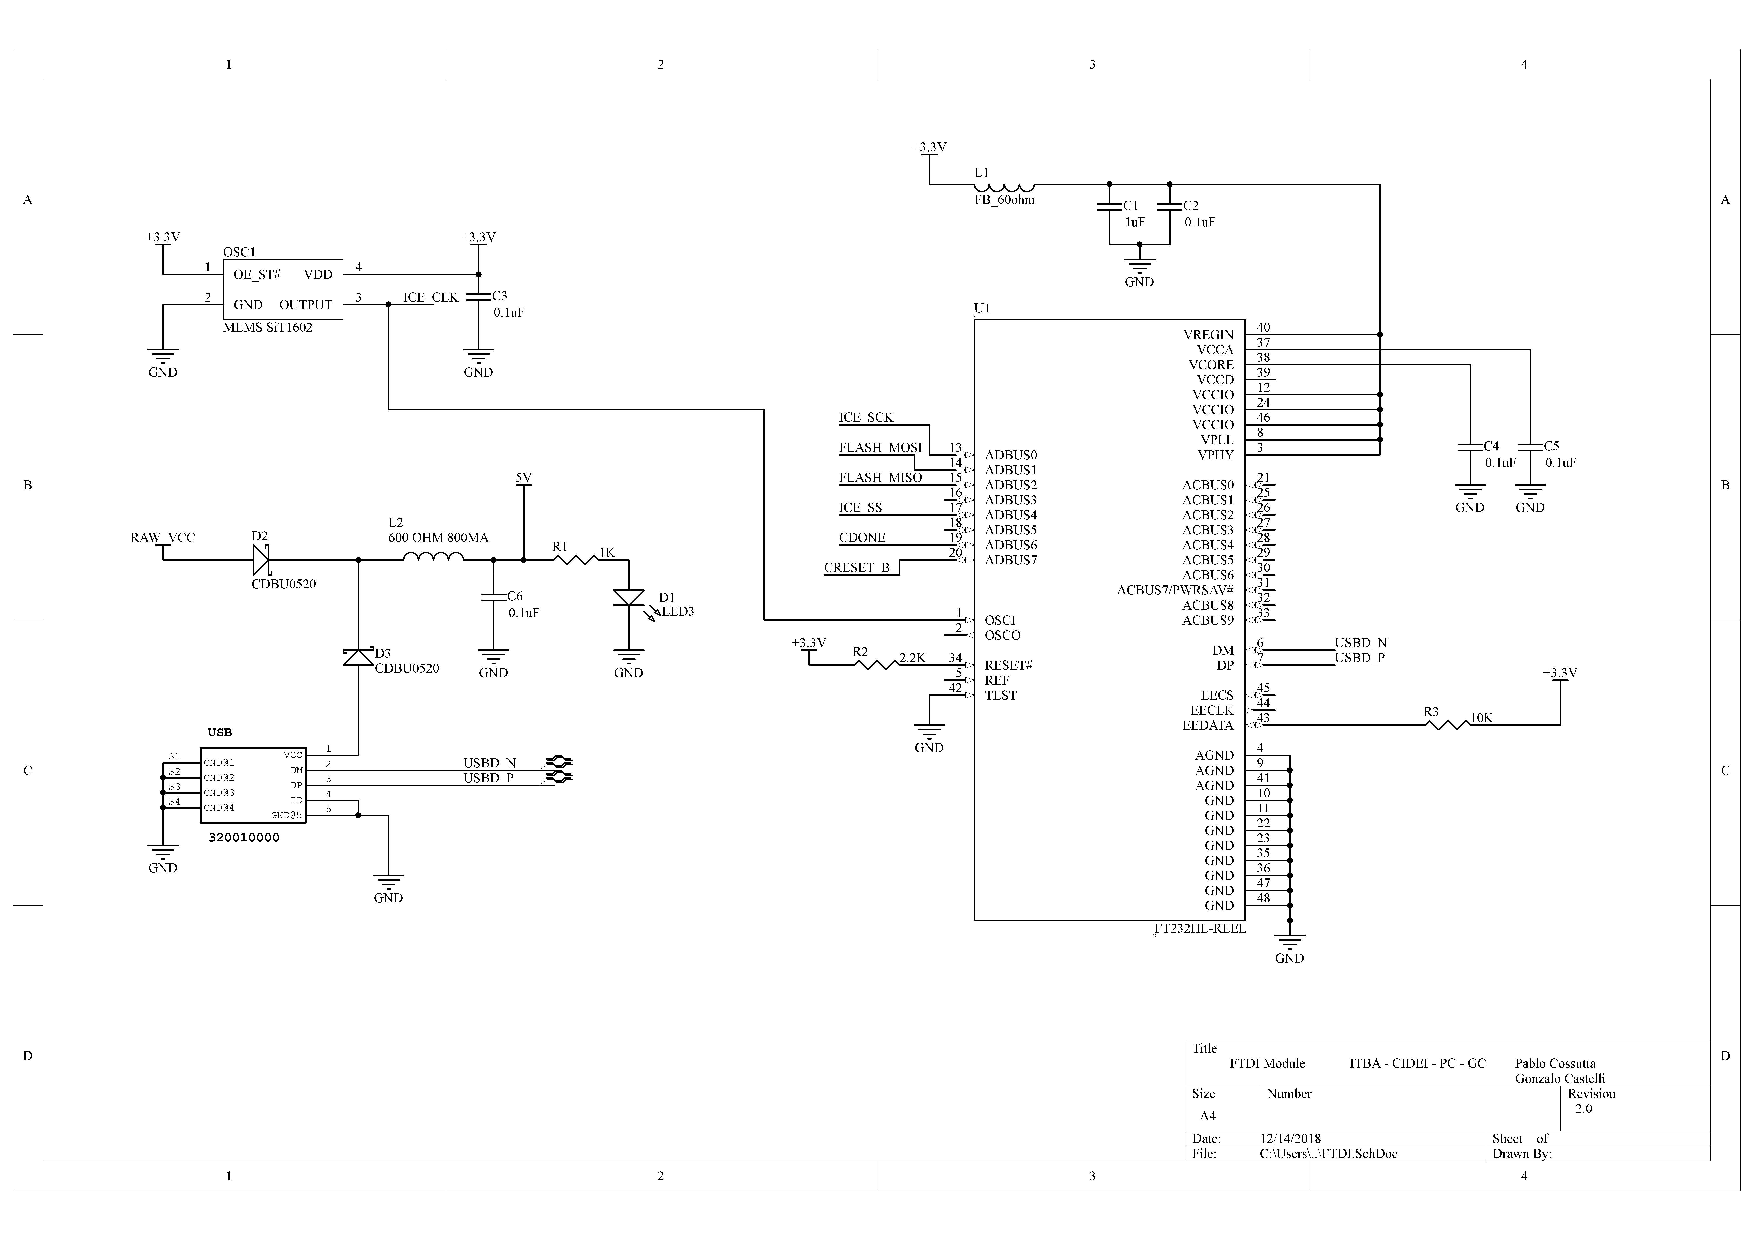
\includepdf[landscape=true]{figs/ftdi.pdf}
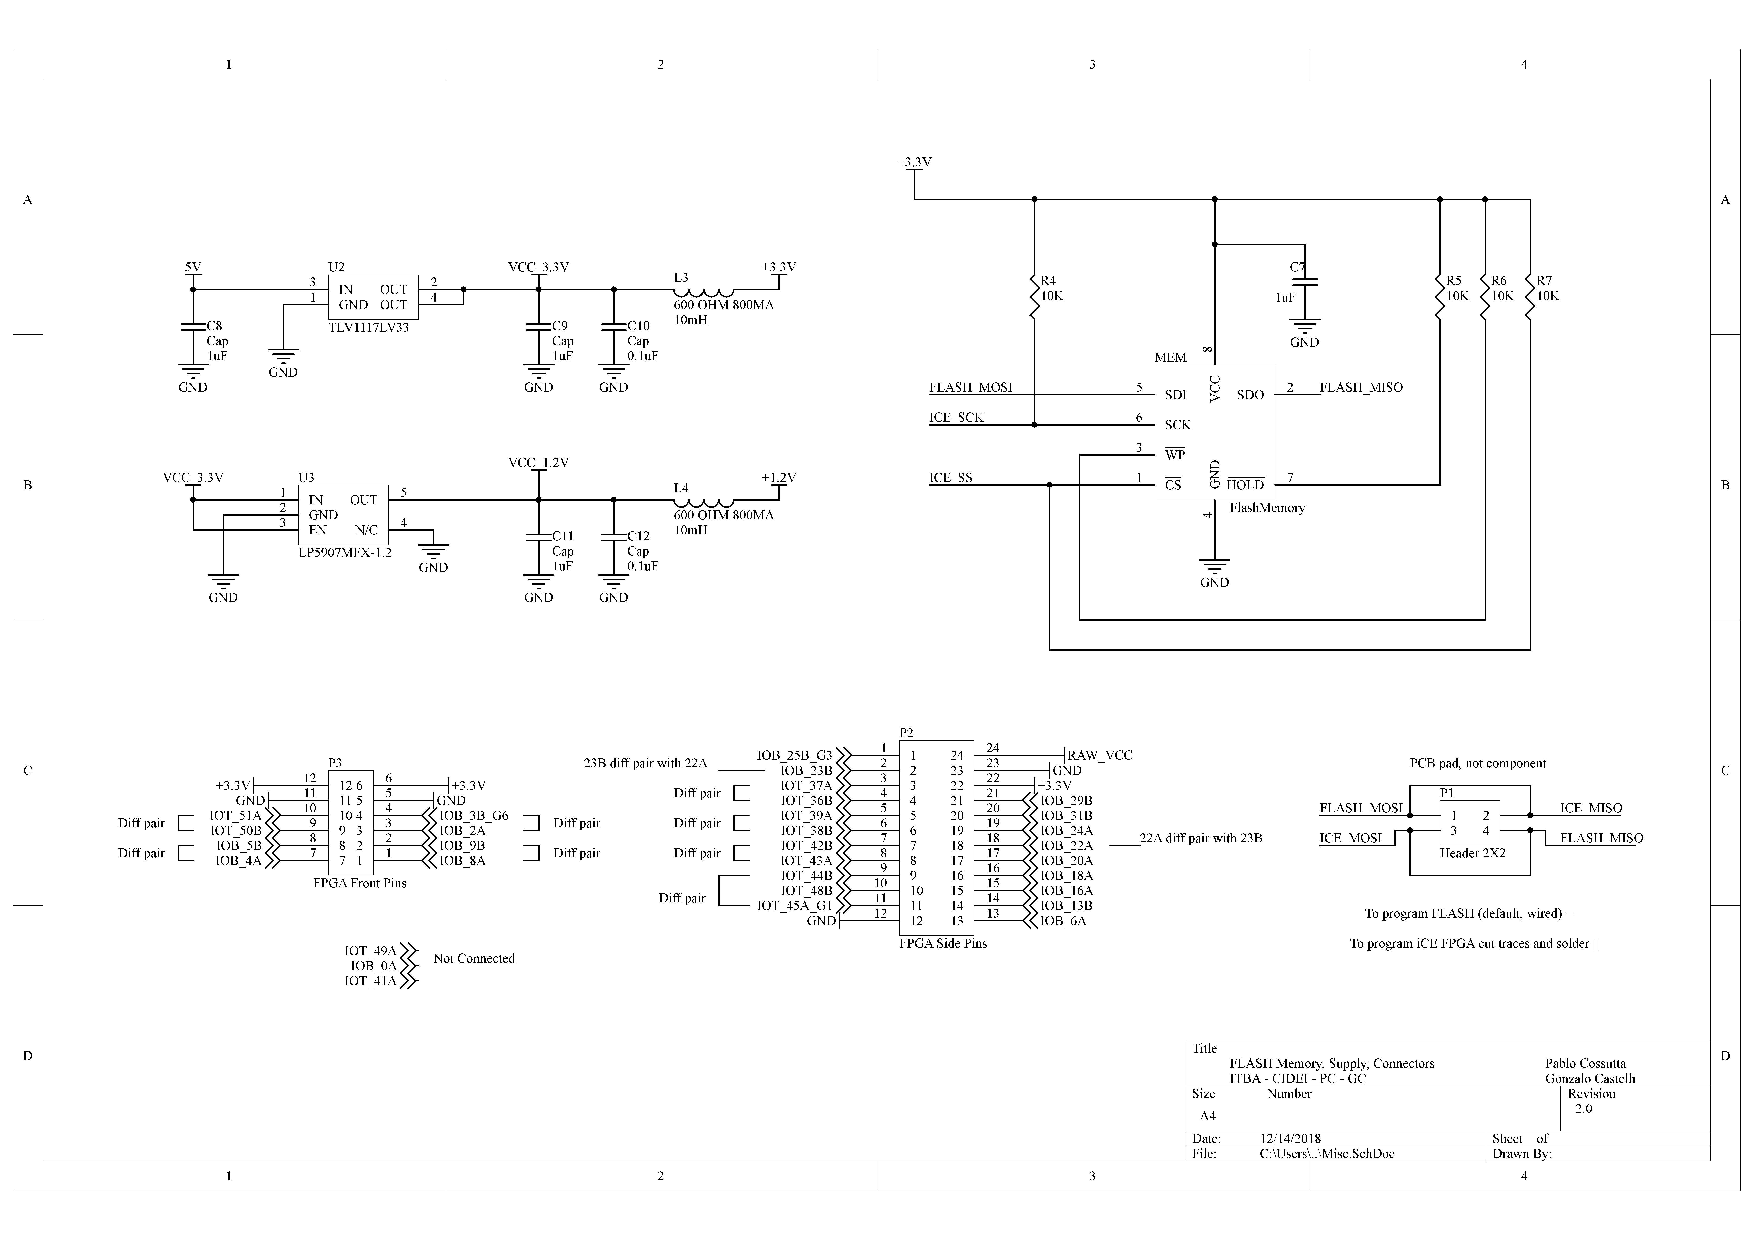
\includepdf[landscape=true]{figs/misc.pdf}
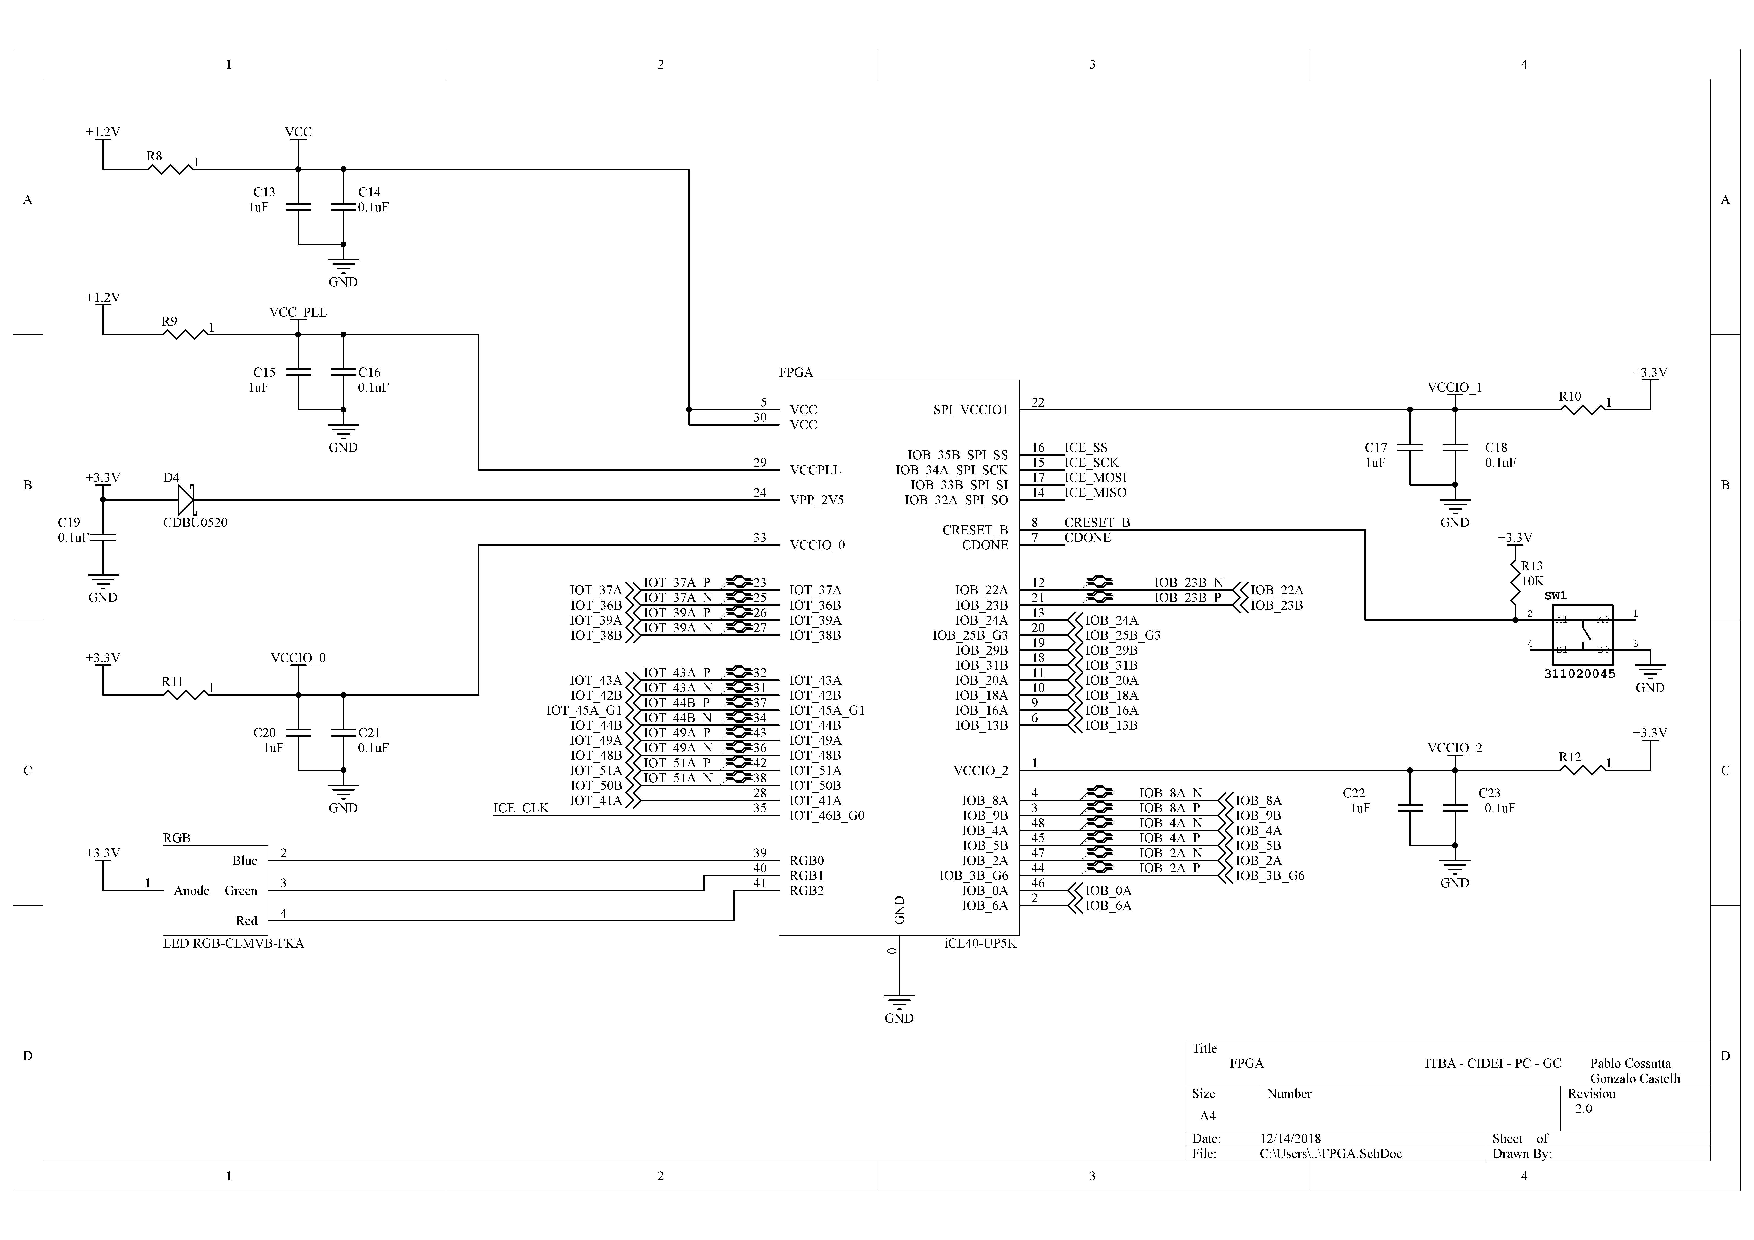
\includepdf[landscape=true]{figs/fpga.pdf}

\section{License}
This project is licensed under a Creative Commons Attribution Share-Alike license, meaning that you are free to use and adapt it for your own needs without asking for permission or paying a fee, even for commercial purposes, as long as you give appropriate credit and release the design under the same license. Visit the
\href{https://creativecommons.org/licenses/by-sa/3.0/}{Creative Commons Website} for further information.

\section{Acknowledgments}
The circuit was inspired by the official manuals and toolchain of the \href{http://www.latticesemi.com/en/Products/DevelopmentBoardsAndKits/iCE40UltraPlusBreakoutBoard.aspx}{iCE40 UltraPlus Breakout Board} from Lattice, and the documentation of the iCE40UP5K FPGA chip.
\end{document}

